\section{Assignment 3.15}

Given a signal amplitude vector x = [3 -1 0.6 -0.8  -2 0 0.9]\\

We first calculate the DFT values by matlab function fft(x).

The results if fft(x) can been seen in figure \ref{fig:opg315} blue dots. Note that only the real values (Amplitudes) are shown for more information see the Matlab file opgave\_315.m.

Now we calculate the twiddle-factor for an N=8 point DFT.
$W_8 = e^(-j*(2*pi*m*n/8)$ where $n$ and $m$ are the matrix notations corresponding to the column, row notation.

We now calculate the needed 8 twiddle-factors corresponding to the 8 different position on the unit circle.\\
${W_8}^0 = 1;$\\
${W_8}^1 = exp((-j*(2*pi/8)));$\\
${W_8}^2 = exp((-j*(2*2*pi/8)));$\\
${W_8}^3 = exp((-j*(2*3*pi/8)));$\\
${W_8}^4 = exp((-j*(2*4*pi/8)));$\\
${W_8}^5 = exp((-j*(2*5*pi/8)));$\\
${W_8}^6 = exp((-j*(2*6*pi/8)));$\\
${W_8}^7 = exp((-j*(2*7*pi/8)));$\\
 
Remember that ${W_8}^n = {W_8}^{n-8}$ for $n>=8$ and so on. 
The full matrix $W$ can bee seen in the matlab file.

We now calculate the product $x*W$ and get the DFT values also seen in the figure \ref{fig:opg315} red dots. 

We observe that the two different methods of calculating DFT values are not the same, this is expected as the vector is a size of 7 elements and the DFT calculated manually is of N=8.

\begin{figure}[H]
    \centering
    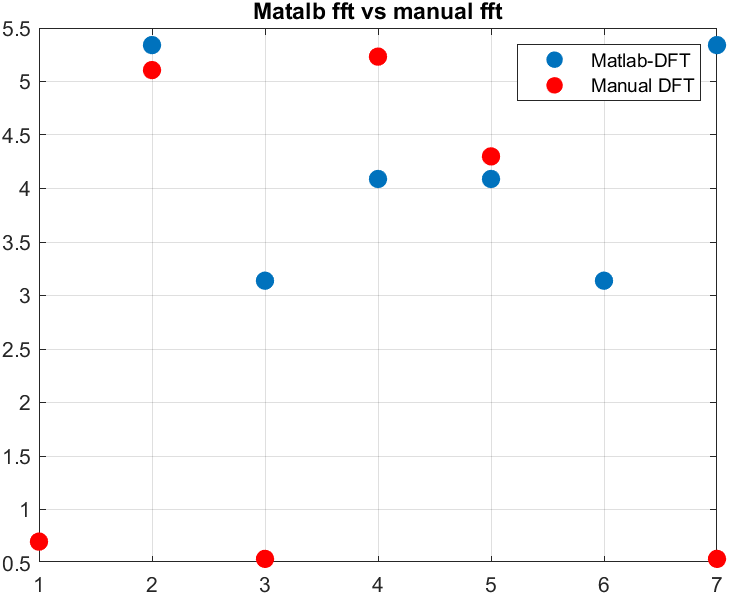
\includegraphics[width=1\textwidth]{matlabStuff/opg315.PNG}
     \caption{Comparison of the matlab DFT (blue) and manual DFT values (red) real values}
    \label{fig:opg315}
\end{figure}